% ============================================================================
% DIAGRAMS & ILLUSTRATIONS
% TikZ-based vector graphics for mathematical concepts
% ============================================================================

\subsection{Grip State Machine Diagram}

\label{fig:grip-state-machine}

\begin{figure}[H]
\centering
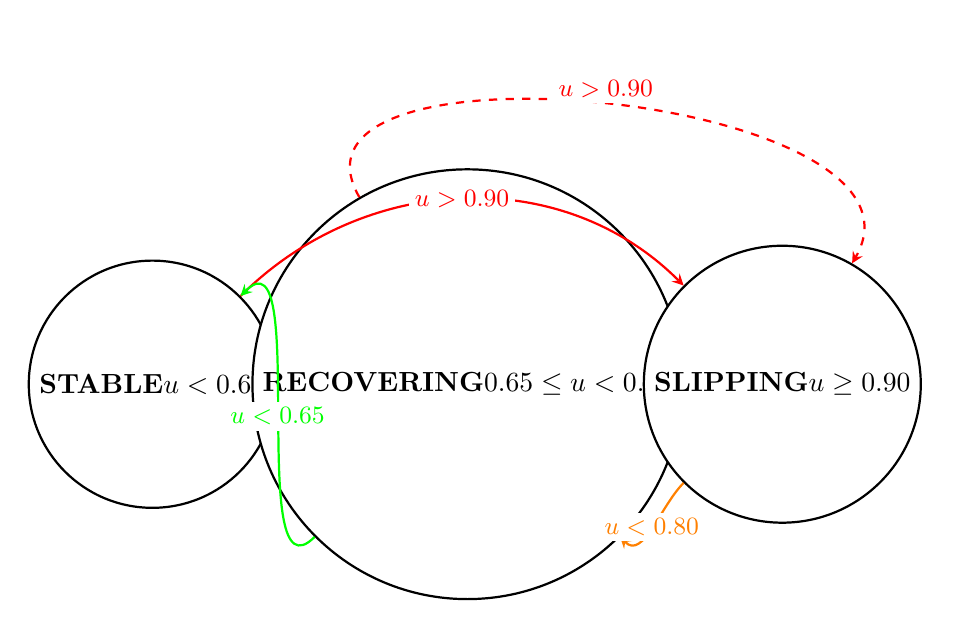
\begin{tikzpicture}[
  state/.style={circle, draw, thick, minimum size=2cm, fill=white},
  arrow/.style={->, thick, >= stealth},
  threshold/.style={midway, fill=white, inner sep=2pt, font=\small}
]

  % States
  \node[state] (stable) at (0, 0) {\textbf{STABLE}\\$u < 0.65$};
  \node[state] (recovering) at (4, 0) {\textbf{RECOVERING}\\$0.65 \le u < 0.90$};
  \node[state] (slipping) at (8, 0) {\textbf{SLIPPING}\\$u \ge 0.90$};

  % Transitions
  \draw[arrow, color=red] (stable) to[out=45, in=135] node[threshold] {$u > 0.90$} (slipping);
  \draw[arrow, color=orange] (slipping) to[out=225, in=-45] node[threshold] {$u < 0.80$} (recovering);
  \draw[arrow, color=green] (recovering) to[out=-135, in=45] node[threshold] {$u < 0.65$} (stable);

  % Hysteresis loop feedback
  \draw[arrow, dashed, color=red, thick] (recovering) to[out=120, in=60] node[threshold, above] {$u > 0.90$} (slipping);

\end{tikzpicture}
\caption{Hysteretic grip state machine. The three-state automaton prevents oscillation at threshold boundaries. Dashed arrow shows direct transition from recovering to slipping if friction utilization increases again.}
\end{figure}

\subsection{Tire Force Vector Diagram}

\label{fig:tire-force-vectors}

\begin{figure}[H]
\centering
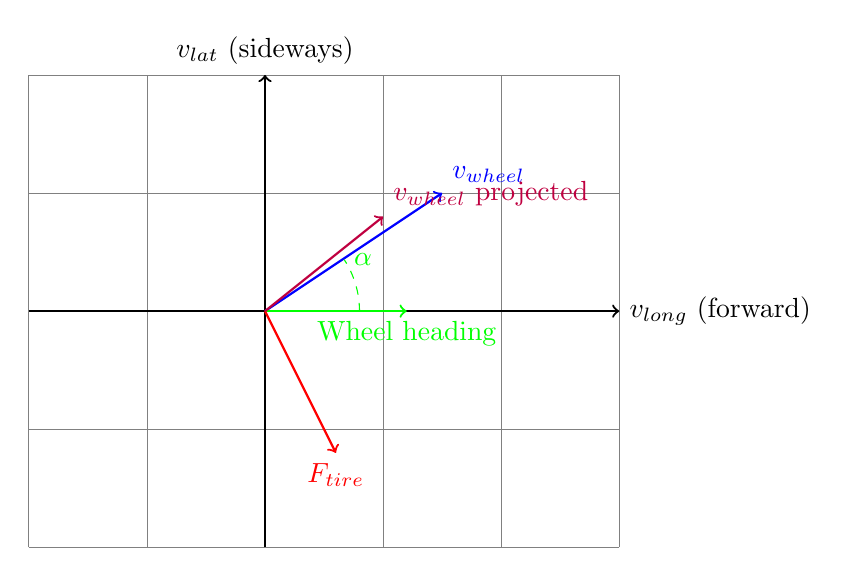
\begin{tikzpicture}[
  scale=1.5,
  axis/.style={thick, ->},
  vector/.style={thick, ->},
  grid/.style={gray, very thin}
]

  % Grid
  \draw[grid] (-2, -2) grid (3, 2);

  % Axes
  \draw[axis] (-2, 0) -- (3, 0) node[right] {$v_{\text{long}}$ (forward)};
  \draw[axis] (0, -2) -- (0, 2) node[above] {$v_{\text{lat}}$ (sideways)};

  % Wheel velocity vector
  \draw[vector, blue, thick] (0, 0) -- (1.5, 1) node[above right, blue] {$\vv{v}_{\text{wheel}}$};

  % Wheel heading vector
  \draw[vector, green, thick] (0, 0) -- (1.2, 0) node[below, green] {Wheel heading};

  % Slip angle arc
  \draw[green, dashed] (0.8, 0) arc (0:33:0.8) node[right, green] {$\alpha$};

  % Force vectors
  \draw[vector, red, thick] (0, 0) -- (0.6, -1.2) node[below, red] {$\vv{F}_{\text{tire}}$};
  \draw[vector, purple, thick] (0, 0) -- (1.0, 0.8) node[above right, purple] {$\vv{v}_{\text{wheel}}$ projected};

\end{tikzpicture}
\caption{Tire force vector diagram showing slip angle $\alpha$ between wheel velocity and heading, and resulting tire force vector that opposes the slip.}
\end{figure}

\subsection{Weight Transfer Diagram}

\label{fig:weight-transfer}

\begin{figure}[H]
\centering
\begin{tikzpicture}[
  scale=2,
  car/.style={rectangle, draw, thick, fill=lightgray, minimum width=2, minimum height=1},
  wheel/.style={circle, draw, thick, fill=black, radius=0.15},
  arrow/.style={->, thick, >= stealth}
]

  % Car body
  \node[car] (car) at (0, 0) {};

  % CoG
  \node[circle, draw, thick, fill=red, minimum size=0.15] (cog) at (0, 0.3) {};
  \node[below=0.3cm of cog, red] {CoG};

  % Wheels
  \node[wheel] (fl) at (-0.9, -0.5) {};
  \node[wheel] (fr) at (0.9, -0.5) {};
  \node[wheel] (rl) at (-0.9, -0.5) {};
  \node[wheel] (rr) at (0.9, -0.5) {};

  % Acceleration arrow
  \draw[arrow, blue, very thick] (0, 0) -- (1.2, 0) node[right, blue] {$a_{\text{long}}$};

  % Weight transfer annotations
  \node[above=0.2cm of fl, red, font=\small] {$N - \Delta W$};
  \node[above=0.2cm of fr, red, font=\small] {$N + \Delta W$};

\end{tikzpicture}
\caption{Weight transfer during longitudinal acceleration. Weight transfers from front to rear. Arrows show acceleration direction.}
\end{figure}

\subsection{Friction Ellipse}

\label{fig:friction-ellipse}

\begin{figure}[H]
\centering
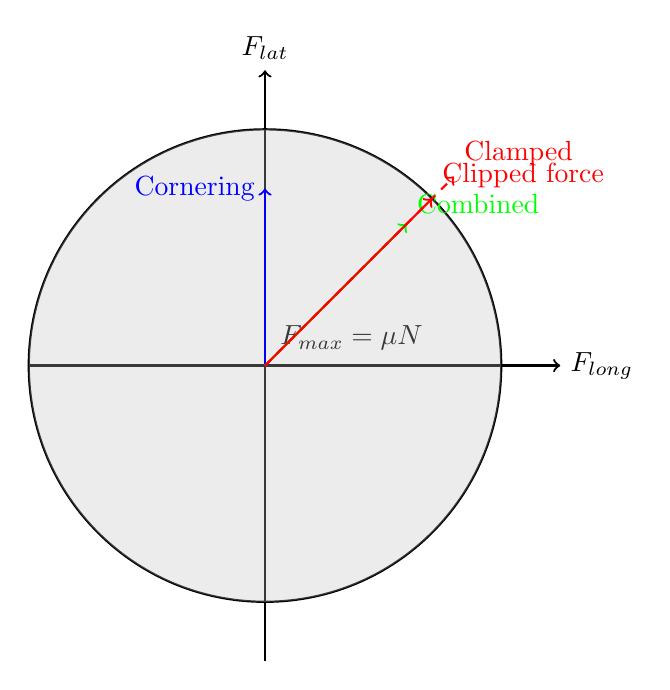
\begin{tikzpicture}[
  scale=1.5,
  axis/.style={thick, ->},
  vector/.style={thick, ->}
]

  % Axes
  \draw[axis] (-2, 0) -- (2.5, 0) node[right] {$F_{\text{long}}$};
  \draw[axis] (0, -2.5) -- (0, 2.5) node[above] {$F_{\text{lat}}$};

  % Friction circle
  \draw[thick, black] (0, 0) circle (2) node[above right=1.8] {$F_{\text{max}} = \mu N$};
  \fill[lightgray, opacity=0.3] (0, 0) circle (2);

  % Example force vectors
  % Cornering only
  \draw[vector, blue, thick] (0, 0) -- (0, 1.5) node[left, blue] {Cornering};

  % Combined slip (within circle)
  \draw[vector, green, thick] (0, 0) -- (1.2, 1.2) node[above right, green] {Combined};

  % Over limit (would be clipped)
  \draw[vector, red, thick, dashed] (0, 0) -- (1.6, 1.6) node[above right, red, dashed] {Clamped};
  \draw[vector, red, thick] (0, 0) -- (1.414, 1.414) node[above right, red] {Clipped force};

\end{tikzpicture}
\caption{Friction ellipse showing maximum available grip circle. Forces exceeding the limit are scaled down to stay within the circle.}
\end{figure}

\subsection{Verlet Integration Particles}

\label{fig:verlet-particles}

\begin{figure}[H]
\centering
\begin{tikzpicture}[
  scale=1.5,
  particle/.style={circle, draw, thick, fill=black, minimum size=0.15},
  vector/.style={->, thick, >= stealth},
  arrow/.style={thick, ->, >= stealth}
]

  % Previous, current, next positions
  \node[particle] (prev) at (0, 0) {};
  \node[above=0.1cm of prev, font=\small] {$\vv{x}_{\text{prev}}$};

  \node[particle] (curr) at (1, 0.3) {};
  \node[above=0.1cm of curr, font=\small] {$\vv{x}_{\text{current}}$};

  \node[particle] (next) at (2.2, 1.2) {};
  \node[above=0.1cm of next, font=\small] {$\vv{x}_{\text{new}}$};

  % Velocity vectors
  \draw[vector, blue] (prev) -- (curr) node[midway, below, blue] {$\vv{v}$};
  \draw[vector, blue, dashed] (curr) -- (1.7, 0.6) node[right, blue] {$\vv{v}$};

  % Acceleration vector
  \draw[vector, red] (1.7, 0.6) -- (2.2, 1.2) node[midway, right, red] {$\vv{a} \cdot dt^2$};

\end{tikzpicture}
\caption{Verlet position update showing how new position is computed from current position, implicit velocity (difference), and acceleration term.}
\end{figure}

\subsection{Car Coordinate System}

\label{fig:car-coordinates}

\begin{figure}[H]
\centering
\begin{tikzpicture}[
  scale=1.5,
  car/.style={rectangle, draw, thick, fill=lightgray, minimum width=1.5, minimum height=1},
  vector/.style={->, thick, >= stealth},
  wheel/.style={circle, draw, thick, fill=black, radius=0.1}
]

  % Car body
  \node[car] (car) at (0, 0) {};

  % Wheels
  \node[wheel] at (-0.7, -0.5) {};
  \node[wheel] at (0.7, -0.5) {};
  \node[wheel] at (-0.7, 0.5) {};
  \node[wheel] at (0.7, 0.5) {};

  % Center of mass
  \node[circle, draw, thick, fill=red, minimum size=0.1] (com) at (0, 0) {};
  \node[below=0.3cm of com, red] {CoG};

  % Heading angle
  \draw[thick, ->] (0, 0) -- (0.7, -0.4) node[right] {$\theta$ (heading)};

  % Forward and right vectors
  \draw[vector, blue, thick] (0, 0) -- (0.6, -0.9) node[below, blue] {Forward};
  \draw[vector, green, thick] (0, 0) -- (0.9, 0.6) node[above, green] {Right};

\end{tikzpicture}
\caption{Car coordinate system with heading angle $\theta$, showing forward and right unit vectors used for slip angle and force calculations.}
\end{figure}

\subsection{Pacejka Curve}

\label{fig:pacejka-curve}

\begin{figure}[H]
\centering
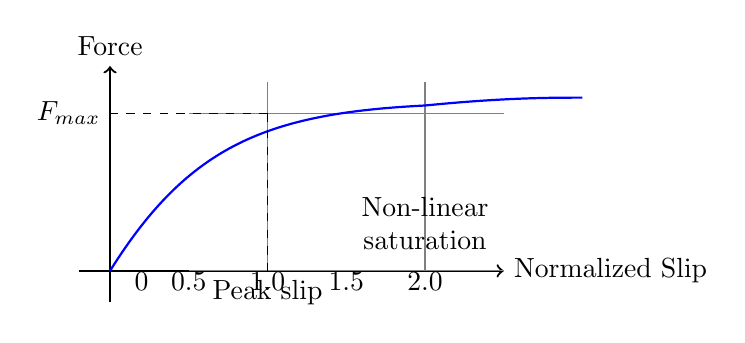
\begin{tikzpicture}[
  scale=2,
  axis/.style={thick, ->}
]

  % Axes
  \draw[axis] (-0.2, 0) -- (2.5, 0) node[right] {Normalized Slip};
  \draw[axis] (0, -0.2) -- (0, 1.3) node[above] {Force};

  % Grid
  \draw[gray, thin] (0.5, 0) grid (2.5, 1.2);

  % Pacejka curve
  \draw[thick, blue] (0, 0) .. controls (0.5, 0.8) and (1, 1) .. (2, 1.05)
                             .. controls (2.5, 1.1) and (2.8, 1.1) .. (3, 1.1);

  % Labels
  \node at (0.2, 0.05) [below] {$0$};
  \node at (0.5, 0.05) [below] {$0.5$};
  \node at (1.0, 0.05) [below] {$1.0$};
  \node at (1.5, 0.05) [below] {$1.5$};
  \node at (2.0, 0.05) [below] {$2.0$};

  % Peak point
  \draw[dashed] (1, 1) -- (1, 0) node[below] {Peak slip};
  \draw[dashed] (1, 1) -- (0, 1) node[left] {$F_{\text{max}}$};

  % Annotation
  \node[text width=2cm, align=center] at (2, 0.3) {Non-linear\\saturation};

\end{tikzpicture}
\caption{Pacejka magic formula characteristic showing nonlinear force response to slip, with saturation at high slip values.}
\end{figure}

\newpage
